\documentclass[a4paper,11pt]{article}
%\documentclass[a4paper,10pt]{scrartcl}
\usepackage{mathtools, nccmath}
\usepackage{tikz-qtree}
\usepackage{lmodern}
\usepackage{amsmath}
\usepackage{mathrsfs}
\usepackage{amssymb}
\usepackage{wasysym}
\usepackage{graphics}
\graphicspath{{images/}}
\usepackage[utf8]{inputenc}

\title{Proofs}
\author{Jason Soegondo}
\date{}

\pdfinfo{%
  /Title    (Proofs)
  /Author   (Jason Soegondo)
  /Creator  (Jason Soegondo)
  /Producer ()
  /Subject  (Mathematics)
  /Keywords (Math, Proofs)
}

\begin{document}
\maketitle
\tableofcontents

\section{Fundamentals}
\subsection{Sets}
Anything can be descripbed as a set or a subset of a larger set.
For example
\begin{itemize}
  \item $0 = \{\O\}$
  \item $1 = \{0\}$
  \item $2 = \{0, 1\}$
  \item $3 = \{0,1,2\}$
  \item $4 = \{0,1,2,3\}$
\end{itemize}
and so on.\medskip\\
For negative numbers you can use any representation you want, its all just an abstraction at the end of the day.
\begin{itemize}
 \item $-1 = \{-0\}$
 \item $-2 = \{-0, -1\}$
 \item $-3 = \{-0, -1, -2\}$
 \item $-4 = \{-0, -1, -2, -3\}$
\end{itemize}
Sets are commonly denoted with a capital character\\
Some common sets are:
\begin{itemize}
 \item{Natural Numbers: $A=\mathbb N$}
 \item{Integers: $A=\mathbb Z$}
 \item{Rational Numbers: $A=\mathbb Q$}
 \item{Real Numbers: $A=\mathbb R$}
 \item{The empty set: $\{\}$ or $\O$}
\end{itemize}
Notation used to describe a value is in a set: $n \in A$\\
If a set is finite, its \textit{cardinality} or \textit{size} is denoted as $|A| = n$\\
\textit{Set-builder notation} is used to describe sets that are too big to list in braces: $E={2n:n \in A}$.\\
In general: $X=\{A(x):P\}$ in words, ``for all A(x) such that \textit{P} is true''\\
Intervals can be described with set-builder notation:
\begin{itemize}
 \item Closed interval: $(a, b)$ = $\{x=\mathbb R:a < x < b\}$
 \item Open interval: $[a, b]$ = $\{x=\mathbb R:a \leq x \leq b\}$
 \item Infinite interval: $(-\infty, b]$ = $\{x=\mathbb R:x \leq b\}$
 \item and the rest
\end{itemize}
\subsubsection{Cartesian Product}
An \textit{ordered pair} is a list $(x, y)$ of two things.\\
The \textit{Cartesian product} of two sets $A$ and $B$ is another set denoted as $A \times B$ which is defined as $A \times B$ = $\{(a, b):a\in A, b\in B\}$\\
Example: $A=\{k,l,m\}$ and $B=\{q,r\}$\\
$A \times B$ = ${(k,q),(k,r),(l,q),(l, r),(m, q),(m,r)}$\vspace{5pt}\\
The set $\mathbb R \times \mathbb R$ is the set of points of the Cartesian plane\\
The set $\mathbb R \times \mathbb N$ would be a bunch of horizontal lines starting from $y=1$\\
And the set $\mathbb N \times \mathbb N$ would just be a bunch of points in the first quadrant of a cartesian plane\vspace{5pt}\\
Cartesian products can be done with more than two sets. The dimensionality of the ordered list would equal the amount of sets multipled together.\vspace{5pt}\\
The Cartesian power $A^n$ is\\ $A^n$ = $A \times A \times A \dots \times A$ = $\{(x_1, x_2, x_3, \dots x_n):x_1,x_2,x_3, \dots x_n \in A\}$
\subsubsection{Subsets}
A set $A$ is a subset of another set $B$ if all elements in $A$ are in $B$: $A \subseteq B$ otherwise, $A \nsubseteq B$.\\
\textbf{Fact}: $\mathbb N \subseteq \mathbb Z \subseteq \mathbb Q \subseteq \mathbb R$\\
\textbf{Fact}: the empty set is a subset of all sets B: $\O \subseteq B$\vspace{5pt}\\
For each element in a set, it can either be in the set or not. Therefore, the amount of subsets that a finite set that has $n$ elements is $2^n$
\subsubsection{Power Sets}
If $A$ is a set, the \textit{power set} is another set denoted as $\mathscr{P}(A)$ and is the set of all subsets of $A$: $\mathscr{P}(A)$ = $\{X: X \subseteq A\}$\vspace{5pt}\\
If $A$ is a finite set then $|\mathscr{P}(A)|$ = $2^{|A|}$ Where $|~|$ denotes cardinality\vspace{5pt}
$\mathscr{P}(\mathbb{R}^{2})$ contains anything that can or will ever be displayed in a 2D plane.
\subsubsection{Set Operations}
The \textit{union} of two sets A and B is: $A \cup B$ = $\{x:x \in A or x \in B\}$\\
The \textit{intersection} of two sets A and B is: $A \cap B$ = $\{x:x \in A and x \in B\}$\\
The \textit{difference} of two sets A and B is: $A - B$ = $\{x:x \in A and x \notin B\}$\vspace{5pt}\\
In other words, $A \cup B$ is the set of all elements in $A$, in $B$, or both. $A \cap B$ is the set of all elements in both $A$ and $B$. $A - B$ is the set of all elements in $A$ but not in $B$\vspace{5pt}\\
Notice that when $A=\{(x, x^{2}):x \in \mathbb{R}\}$ and $B=\{(x, x+2):x \in \mathbb{R}\}$; in other words, when A and B are a set of function input and output pairs, $A \cap B$ is a set containing the point(s) of intersection between the two functions.\bigskip\\
Two sets, $A$ and $B$ are said to be disjoint sets if they share no elements in common.
\subsubsection{Complement}
A \textit{universal set} is a set that another set would naturally be the subset of. Sets like $\mathbb N$, $\mathbb R$, $\mathbb Q$ and more are considered universal sets.\vspace{5pt}\\
The \textit{complement} of the set $A$ whose universal set is $U$ would be $\bar{A}=U-A$
\subsubsection{Indexed Sets}
\[\bigcap_{i=1}^{n}A_{i}=A_1 \cap A_2 \cap A_3 \cap A_4 \dots \cap A_n=\{x:x \in A_i, for~1 \leq i \leq n\}\]
where $x$ is in ever set $A_i$
\[\bigcup_{i=1}^{n}A_{i}=A_1 \cup A_2 \cup A_3 \cup A_4 \dots \cup A_n=\{x:x\in A_i, for~1 \leq i \leq n\}\]
where $x$ is in at least one set $A_i$\vspace{5pt}\\
Given $A_i$ for $i \in I$ where $I$ is the set of possible subscripts, The set $I$ is called the \textit{index set}. We can rewrite the above using indexed notation:\vspace{5pt}\\
$\bigcap_{i \in I}^{n}A_{i}=A_1 \cap A_2 \cap A_3 \cap A_4 \dots \cap A_n=\{x:x \in A_i$ for every set $A_i$, for $1 \leq i \leq n\}$\vspace{8pt}\\
$\bigcup_{i \in I}^{n}A_{i}=A_1 \cup A_2 \cup A_3 \cup A_4 \dots \cup A_n=\{x:x\in A_i,$for at least one set $A_i$, for $1 \leq i \leq n\}$
\subsubsection{Zermelo-Fraenkel Axioms}
\begin{itemize}
 \item \textit{Well-ordered Principle}: a set is considered well-ordered if each non-empty subset has a smallest number
 \item \textit{Axiom of Foundation}: For all non-empty sets $X$,\\
 $\exists x \in X$ such that $X \cap x = \O$. Remember that elements are defined as sets eg: $4=\{0,1,2,3\}$. So, it follows that $x$ must be the smallest element, because the proposition $X \cap x=\O$ only holds for the smallest element in $X$. This axiom also rules out circularly defined ``sets'' such as $A=\{A\}$
\end{itemize}
\subsection{Logic}
Quick section for anything new. READ THE LOGIC NOTES for more details about propositional logic.
\subsubsection{Quantifiers}
$\forall$ represents phrase `for all' or `for each'. called the \textit{universal qualifier}\\
$\exists$ represents phrase `there exists' or `there is a'. called the \textit{existential qualifier}
\subsubsection{English to Symbolic Logic}
Given a set $X$ and $Q(X)$ a proposition about $x$. The following statements mean the same thing:
\begin{itemize}
 \item $\forall x \in X, Q(x)$
 \item $(x \in X) \rightarrow Q(X)$
\end{itemize}
In english:
\begin{itemize}
 \item for all $x$ in $X$, $Q(x)$
 \item if $x$ is in $X$, then $Q(x)$
\end{itemize}
Oftentimes it is more practical to think of a universally quantified statement as a conditional.
\subsubsection{Logical Inference}
Assuming that the given proposition is actually true, we can make inferences given certain information:
\begin{itemize}
 \item \textit{Modus Ponens}: $(P \rightarrow Q)$, given $P$, we can infer $Q$
 \item \textit{Modus Tollens}: $(P \rightarrow Q)$, given $\neg Q$, we can infer $\neg P$
 \item \textit{Elimination}: $(P \vee Q)$, given $\neg P$, we can infer $Q$
\end{itemize}
\subsubsection{Closing Notes}
Logic is important because:
\begin{itemize}
 \item Truth tables tell us the exact meaning of words such as ``and'' and ``or''. Logic also tells us exactly what constructs like ``if...then'' mean.
 \item Rules of inference provide a system in which we can produce new information(propositions) from known information.
 \item Logical rules like De Morgan's laws help us to correctly change the forms of certain propositions to potentially make them more useful.
\end{itemize}
\section{Counting}
\subsection{Multiplication Principle}
A list $(a, b, c)$ where $a$, $b$, $c$ can have $a_i$, $b_i$, $c_i$ different choices for each value respectively, can form multiple unique lists. The amount of unique lists that can be formed can be found using the \textit{Multiplication Principle}.\vspace{5pt}\\
\textbf{Definition}\\
Given a list of length $n$, there are $a_1$ possible choices for the first entry, $a_2$ possible choices for the second entry, and so on. The total number of different lists that can be made this way is the product $a_{1}*a_{2}*a_{3} \dots *a_{3}$
\begin{figure}[h]
 \centering
 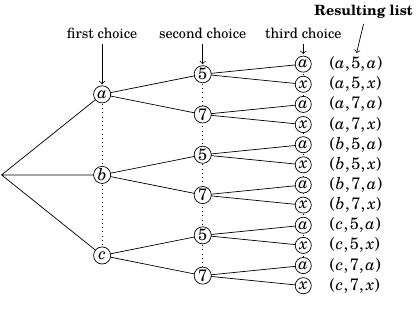
\includegraphics[width=0.75\textwidth]{multiprinc.png}
 \caption{A tree showing how the multiplication principle works}
\end{figure}
\subsection{Addition and Subtraction Principle}
\textbf{Addition Principle}\\
Given a finite set $X$, $X$ can be decomposed as a union\\
$X=X_1 \cup X_2 \cup X_3 \dots \cup X_n$ whenver $X_i \cap X_j = \o$ whenever $i \neq j$.\\
In otherwords, each set does not share an element with any other set.\vspace{5pt}\\
Then, $|X|=|X_1|+|X_2|+|X_3|...+|X_4|$\vspace{5pt}\\
\textbf{Example}\\
Suppose you want to find how many strings of \textit{length} 4 made up of the letters $a,b,c,d,e,f,g$ contain the letter \textit{e}. You would start by arranging it into 4 possibilites\vspace{5pt}\\
\begin{tabular}{|c|c|c|c|c|}
\hline
 $X_1$ & e & \ & \ & \ \\
 \hline
 $X_2$ & \ & e & \ & \ \\
 \hline
 $X_3$ & \ & \ & e & \ \\
 \hline
 $X_4$ & \ & \ & \ & e \\
\hline
\end{tabular}\vspace{5pt}\\
Using the multiplication principle we can find the amount of unique lists that could be made out of each possibility\vspace{5pt}\\
\begin{tabular}{|c|c|c|c|c|c|}
 \hline
 $X_i$ & \ & \ & \ & \ & $|X_i|$\\
 \hline
 $X_1$ & 1 & 6 & 5 & 4 & 120\\
 \hline
 $X_2$ & 6 & 1 & 5 & 4 & 120\\
 \hline
 $X_3$ & 6 & 5 & 1 & 4 & 120\\
 \hline
 $X_4$ & 6 & 5 & 4 & 1 & 120\\
\hline
\end{tabular}\vspace{5pt}\\
Finally, using the \textit{addition principle} add up the cardinality of the 4 subsets to find the cardinality of the set $X$ of unique 4 character strings that can be made using only the letters $a,b,c,d,e,f,g$ and contain $e$.\vspace{5pt}\\
\textbf{Subtraction Principle}\\
Given $X$ is a subset of a finite set $U$, remember that the complement \\of $X$, is $\bar{X}=U-X$. It follows that $|\bar{X}| = |U|-|X|$.\vspace{5pt}\\
In otherwords, if $X \subseteq U$, then $|U-X| = |U|-|X|$\vspace{5pt}\\
\textbf{Example}\\
Suppose you want to find how many strings of length 4 made up of the letters $a,b,c,d,e,f,g$ contain the letter $e$ with repitition allowed;\\that is, letters can be used multiple times)\vspace{5pt}\\
Using the multiplication principle, we can find the set of unique 4 character strings that can be made using the letters $a,b,c,d,e,f,g$: $7^4=2401$.\vspace{5pt}\\
\begin{tabular}{|c|c|c|c|c|}
 \hline
 7 & 7 & 7 & 7 & 2401\\
 \hline
\end{tabular}\vspace{5pt}\\
We can also find the set of unique 4 character strings that only do not contain $e$, but contain $a,b,c,d,f,g$: $6^4 = 1296$\vspace{5pt}\\
\begin{tabular}{|c|c|c|c|c|}
 \hline
 6 & 6 & 6 & 6 & 1269\\
 \hline
\end{tabular}\vspace{5pt}\\
Finally using the subtraction principle we can take the \textit{difference} between the two sets, $2401-1296=1105$, which results in a set of unique 4 character strings that contain $e$.
\subsection{Factorials}
Given $n$ is a non-negative integer, $n!$ is the number of lists of length $n$ that can be made from $n$ symbols, without repitition.\vspace{5pt}\\
\begin{tabular}{|c|c|c|}
 \hline
 $0!$ & () & 1\\
 \hline
 $1!$ & a & 1\\
 \hline
 $2!$ & ab ba & 2\\
 \hline
 $3!$ & abc acb bac bca cab cba & 6\\
 \hline
 $\vdots$ & $\vdots$ & $\vdots$\\
 \hline
\end{tabular}\vspace{5pt}\\
As seen above, factorials can be calculated using the multiplication principle.\vspace{5pt}\\
\textbf{Proof}\\
$0!=1$ must be true because the generalized equation for a factorial is $n!=n(n-1)!$. If $0!=0$ then $1!=0$ which is obviously wrong, so $0!=1$ must be true.
\subsubsection{Permutations}
In general a set of $n$ elements will have $n!$ amount of permutations.\\
A \textit{permutation} of $X$ is a non-repetitive list made from all elements of $X$.\\
A \textit{k-permutation} of $X$ is a non-repetitive list made from $k$ elements of $X$.\vspace{5pt}\\
For example: the amount of non-repetitive lists made from two elements of a set $\{a, b, c, d\}$ is 12 because using the multiplication principle, there are 4 choices for the first element and 3 choices for the second element: $3*4=12$
\begin{center}
  $ab$ $ac$ $ad$ $ba$ $bc$ $bd$ $ca$ $cb$ $cd$ $da$ $db$ $dc$
\end{center}
\textbf{Notation}:\\
$P(n,k)$ represents the number of \textit{k}-permutations of a set of size $n$\\
For example:\\
$P(4,5)=0$\\
$P(2,0)=1$, here the empty list $()$ is the only possible permutation\vspace{5pt}\\
\textbf{Definition}:\\
$P(n,k)=n(n-1)(n-2)...(n-k+1)$\\
if $0 \leq k \leq n$ then the above can be rewritten as:\\$P(n,k)=\frac{n!}{(n-k)!}$
\subsection{Counting Sets}
When permuting a \textit{list}, changing the position of an element creates a new list eg: $ab$ and $ba$ are two different permutations. The same cannot be said when permuting subsets where it would only results in a single subset $\{a, b\}$\vspace{5pt}\\
Take $A=\{a, b, c, d, e\}$, $P(5, 2)=20$ possible lists.
\begin{center}
  $ab$ $ac$ $ad$ $ae$ $ba$ $bc$ $bd$ $be$ $ca$ $cb$ $cd$ $ce$ $da$ $db$ $dc$ $de$ $ea$ $eb$ $ec$ $ed$
\end{center}
But $A$ only has $10$ subsets
\begin{center}
 $\{a,b\}$ $\{a,c\}$ $\{a,d\}$ $\{a,e\}$ $\{b,c\}$ $\{b,d\}$ $\{b,e\}$ $\{c,d\}$ $\{c,e\}$ $\{d,e\}$
\end{center}
\textbf{Definition}\\
Given that $n$ and $k$ are integers, $(^{n}_{k})$ denotes the number of subsets that can be made by choosing $k$ elements of an n-element set.\vspace{5pt}\\
Notice that $~(^{n}_{k})*k!=P(k)$\\because each subset has $k!$ possible permutations.\vspace{2pt}\\
substitute: $~(^{n}_{k})*k!=\frac{n!}{(n-k)!}$\\
thus, $~~~~~~~~~(^{n}_{k})=\frac{n!}{k!(n-k)!}$
\subsection{Pascal's Triangle and the Binomial Theorem}
Notice the pattern: $(^{n+1}_k)=(^n_{k-1})+(^n_k)$\vspace{5pt} given $1 \leq k \leq n$\\
To understand this, think of $(^{n+1}_k)$ as the amount of \textit{k-subsets} resulting from the set $A=(0,1,2,3\dots n)$.
$(^n_k)$ is the amount of \textit{k-subsets} resulting from the set $(1,2,3\dots n)$; in other words, $(^n_k)$ counts the subsets of $A$ that \textbf{do not} contain $0$.
$(^n_{k-1})$ is the amount of subsets of $A$ that \textbf{do} contain $0$ because if you were to start each subset with $\{0\}$, you can append an additional $k-1$ elements to each subset.\vspace{5pt}\\
Pascal's triangle can be written with this pattern in mind.
\begin{center}
 $1$\\
 $1~1$\\
 $1~2~1$\\
 $1~3~3~1$\\
 $1~4~6~4~1$\\
 $1~5~10~10~5~1$
 \vspace{5pt}\\
 $(^0_0)$\\
 $(^1_0)~(^1_1)$\\
 $(^2_0)~(^2_1)~(^2_2)$
\end{center}
The binomial theorem can also be written with this pattern in mind.\vspace{5pt}\\
$(x+y)^n=(^n_0)x^n+(^n_1)x^{n-1}y+(^n_2)x^{n-2}y^2\dots+(^n_{n-1})xy^{n-1}+(^n_n)y^n$
\subsection{Inclusion-Exclusion Principle}
\begin{figure}[h]
 \centering
 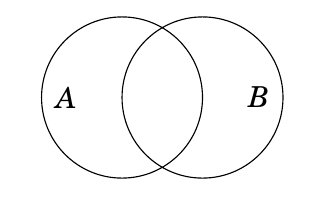
\includegraphics[width=0.40\textwidth]{venn.png}
\end{figure}
The cardinality $|A \cup B|$ is relatively easy to find. $|A|+|B|$ is close, but not quite because it does not exclude the elements in \textbf{both} $A$ and $B$.\\
\textbf{Definition}: $|A \cup B|=|A|+|B|+|A \cap B|$\vspace{5pt}\\
\textbf{Example}\\
A hand of 3-card hand is dealt from a standard deck of 52 cards. How many hands have all red or all face cards?
\begin{enumerate}
 \item Let $|A|$ = the amount of possible 3-card hands that contain all red cards
 \item Let $|B|$ = the amount of possible 3-card hands that contain all face cards
 \item $|A|=(^{26}_3)$
 \item $|B|=(^{12}_3)$
 \item Since you can freely rearrange a hand, we will consider them as sets as opposed to lists.
 \item The deck only has 6 red faced cards, so $|A \cap B|=(^{6}_3)$.
 \item Using the equation derived previously, $|A \cup B|=(^{26}_3) + (^{12}_3) - (^{6}_3)$
\end{enumerate}
\begin{figure}[h]
 \centering
 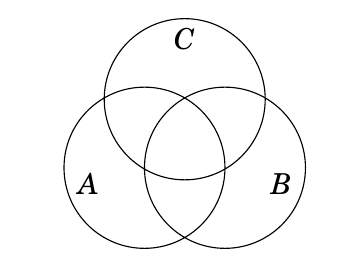
\includegraphics[width=0.40\textwidth]{trivenn.png}
\end{figure}
$|A \cup B \cup C|=|A|+|B|+|C|-|A \cap B|-|A \cap C| - |B \cap C| + |A \cap B \cap C|$\\
Looking at the venn diagram above, this equation can easily be derived.
\subsection{Counting Multisets}
Multisets are sets that contain duplicate elements. The \textbf{cardinality} of the set $A$, $|A|$ is the amount of elements in the set while
the \textbf{multiplicity} of $x \in A$ is the amount of times $x$ appears in $A$.\vspace{5pt}\\
Although there are no \textit{subsets} of cardinality 5 in the set $X=\{a, b,c, d, e\}$, there are multiple multisets of cardinality 5 from $X$\\
eg: $\{a, a, a, a, a\}~~\{a, a, b, c, d, e\}~~\{b,b,b,b,b\}~~$etc.\vspace{5pt}\\
The amount of multisets that can be created from a list can be described using the following diagram.
Take the case of $X=\{a, b, c, d\}$.\vspace{5pt}\\
\begin{tabular}{|c|}
\hline
Multisets\\
\hline
$aa|b|c|d$\\
$a|bb|c|d$\\
$a|bb|cc|d$\\
$aaa|||dd$\\
$aaaaa|||$\\
\hline
\end{tabular}\vspace{5pt}\\
If the list keeps going we end up with $(^8_3)=\frac{8!}{3!(5)!}=56$.\\
Notice that all \textit{k-element} multisets of $X$ can be represented using $k$ elements and $n-1$ bars separating each unique element.\vspace{2pt}\\
$****|****|**** \dots |****$\\
with $k$ stars and $n-1$ bars separating the stars into $n$ groups.\vspace{5pt}\\
\textbf{Definition}\\
In general, the \textit{k-multiset} of a set with $n$ elements is:
\begin{center}
$(^{k+n-1}_{n-1})$.
\end{center}
Rather than treating each element as a numerical value, think of $k+n-1$ as the possible positions that the bar($|$) can be placed on the set, $\{@@@@@@@@\}$ where each symbol represents a location on the multiset of size $k$.\vspace{5pt}\\
\textbf{Definition}\\
If a multiset with $n$ values has $p_1, p_2, p_3 \dots p_k$ multiplicities. The total number of permutations possible on the multiset is:
\begin{center}
\large{$\frac{n!}{p_1!~p_2!~p_3! \dots p_k!}$}
\end{center}
For example, BANANA is a multiset where $p_1=1$, $p_2=3$, $p_3=2$. Using the equation above, the amount of permutations of BANANA is $\frac{6!}{3!~2!}=60$.\vspace{5pt}\\
The idea behind the formula is to remove the amount of permutations where repeated characters are swapped with one another from the total number of permutations($n!$).
Given an element with a \textit{multiplicity} of $k$, there are $k!$ ways to permute said elements in their given positions eg: the A in BANANA has a multiplicty of $3$ and therefore, $3!$ in place permutations:\vspace{10pt}\\
\begin{tabular}{|c|}
\hline
BA$_1$NA$_2$NA$_3$\\
BA$_2$NA$_1$NA$_3$\\
BA$_3$NA$_2$NA$_1$\\
BA$_1$NA$_3$NA$_2$\\
BA$_2$NA$_3$NA$_1$\\
BA$_3$NA$_1$NA$_2$\\
\hline
\end{tabular}\vspace{10pt}\\
For N in BANANA it's $2!$\vspace{10pt}\\
\begin{tabular}{|c|}
\hline
BAN$_1$AN$_2$A\\
BAN$_2$AN$_1$A\\
\hline
\end{tabular}\vspace{10pt}\\
Combining the two multiplicites, $2!3!=12$\vspace{10pt}\\
\begin{tabular}{|c|}
\hline
BA$_1$N$_1$A$_2$N$_2$A$_3$\\
BA$_2$N$_1$A$_1$N$_2$A$_3$\\
BA$_3$N$_1$A$_2$N$_2$A$_1$\\
BA$_1$N$_1$A$_3$N$_2$A$_2$\\
BA$_2$N$_1$A$_3$N$_2$A$_1$\\
BA$_3$N$_1$A$_1$N$_2$A$_2$\\
\hline
BA$_1$N$_2$A$_2$N$_1$A$_3$\\
BA$_2$N$_2$A$_1$N$_1$A$_3$\\
BA$_3$N$_2$A$_2$N$_1$A$_1$\\
BA$_1$N$_2$A$_3$N$_1$A$_2$\\
BA$_2$N$_2$A$_3$N$_1$A$_1$\\
BA$_3$N$_2$A$_1$N$_1$A$_2$\\
\hline
\end{tabular}\vspace{10pt}\\
This pattern holds true for all unique permutations of the multiset. In conclusion, permutations of BANANA can be placed into groups of $12$ \textbf{repeated} permutations; that is, $\frac{6!}{2!3!}=\frac{720}{12}$ gives us the amount of \textbf{unique} permutations. Or more generally $\frac{n!}{p_1!p_2!...p_k!}$

\subsection{Division and Pigeonhole Principles}
Given a number $x$, its \textit{floor}, $\lfloor x \rfloor$ is the number rounded \textbf{down} to the nearest integer. The ceiling, $\lceil x \rceil$ is the number rounded \textbf{up} to the nearest integer.
\subsubsection{Pigeonhole Principle}
There are $n$ pigeons in $k$ pigeonholes. Some of the $k$ boxes may contain more than one pigeon, but the average number of pigeons per box must be $\frac{n}{k}$.
Obviously one or more boxes contain at least $\lceil \frac{n}{k} \rceil$ or more pigeons. Similarly, at least one or more boxes contain at least $\lfloor \frac{n}{k} \rfloor$ or less pigeons.\vspace{5pt}\\
\textbf{Division Principle}\\
Supposed $n$ objects are placed in $k$ boxes.\\
Then at least one box contains $\lceil \frac{n}{k} \rceil$ or more objects\\
and at least one box contains $\lfloor \frac{n}{k} \rfloor$ or fewer objects.\vspace{5pt}\\
\textbf{Pigeonhole Principle}\\
If $n>k$ then at least one box contains more than one object\\
\hspace*{10pt}(because $\frac{n}{k} < 1)$)\\
If $n<k$ then at least one box is empty\\
\hspace*{10pt}(because $\frac{n}{k} < 1)$)\vspace{5pt}\\
\textbf{Example}\\
Pick six numbers out of $[0,9]$. Prove that in any combination of the six numbers, there will be two numbers that sum up to 9.\\
List all possible sum of two numbers (in the range) that add to 9:\\
$(0,9)(1,8),(2,7),(5,4),(6,3)$\\
Notice that there are only 5 possible ``boxes''. No matter what 6 numbers we choose, $\frac{5}{6} < 1$. Which means that at least one box will have more than 1 number. So we have proven the above conjecture.
\section{Proofs}
\subsection{Direct Proofs}
\textbf{Example}\\
Prove that $2\sqrt{xy} \leq x + y$ given $x,y \in \mathbb{N}$.\vspace{5pt}\\
\textbf{Proposition}: $2\sqrt{xy} \leq x + y$\vspace{5pt}\\
\textit{Proof}
\begin{itemize}
  \item Notice that $0 \leq (x - y)^2$, that is $0 \leq x^2-2xy+y^2$ is true by a given axiom.
  \item Adding $4xy$ to both sides, we get $4xy \leq x^2+2xy+y^2$, that is $4xy \leq (x+y)^2$
  \item Square root both sides: $2\sqrt{xy} \leq x+y$ $~~~~~~~~~\blacksquare$
\end{itemize}
\subsubsection{Steps to a Direct Proof}
\begin{enumerate}
 \item Note the definitions of each part of the proposition eg: what set a variable is in, whether it's positive, negative, etc.

 \item Remember certain axioms that may be useful for the proof eg: the definition of an even number is $x=2z$ for $z \in \mathbb{Z}$, etc.

 \item Initially, it may be a good idea to write down the first and last lines of the proof first, so that you know the ``start'' and the ``endgoal''.

 \item If a proposition seems obviously true, it may be easier to prove the proposition by working backwards such as in the proof of $2\sqrt{xy} \leq x+y$.\vspace{5pt}\\
 You can start by squaring both sides resulting in $4xy \leq x^2 + 2xy + y^2$. Then, subtracting $4xy$ from both sides we get $0 \leq (x-y)^2$ which is true by another axiom.
\end{enumerate}
\subsubsection{Notes on Working Backwards}
In short, a proof by working backwords starts by \textit{assuming} that the proposition is true.\\ If that is the case, then there must be a process in which the proposition can be transformed into another proposition that we know to be true.\\
Reverse the process and you get the proof.
\subsubsection{Cases}
Sometimes a proof may have multiple cases such as the proof that the  expression $1+(-1)^n(2n-1)$ is a multiple of 4. Just looking at the expression you can kind of guess that the two cases are the scenarios where $n$ is either even or odd.\vspace{5pt}\\
\textbf{Proof} If $k$ is a multiple of $4$, then $1+(-1)^n(2n-1)=k$\vspace{5pt}\\
\textbf{case} $n=2n$ (even)\\
$1+(-1)^{(2n)}(2(2n)-1)=k$\\
notice $-1^{2n} = 1$\\
$1+(4n-1)=k$\\
$4n=k$
\vspace{5pt}\\
\textbf{case} $n=2n+1$ (odd)\\
$1+(-1)^{(2n+1)}(2(2n+1)-1)=k$\\
notice $-1^{2n+1} = -1$\\
$1-(4n+1)=k$\\
$-4n=k$\vspace{5pt}\\
Sometimes cases are so similar that you can omit the second proof and say that ``Without loss of generality...''
\subsection{Contrapositive Proof}
A contrapositive proof in short is that $P \rightarrow Q$ is equivalent to $\neg P \rightarrow \neg Q$. Keep \textit{De Morgan's Law} in mind when doing a contrapositive proof. $\neg (P \wedge Q)$ is equivalent to $\neg P \vee \neg Q$\bigskip\\
Integers $a$ and $b$ are congruent modulo $n$, $a \equiv b$(mod $n$). If $n | (a-b)$. This is the same as saying that $n | a$ and $n | b$ have the same remainder.

\subsection{Proof by Contradiction}
We can prove an if-then statement by assuming the opposite of the proposition. If the assumtion leads to a contradiction, then we know that the statement must be true.\medskip\\
Example:\\
$a \rightarrow b$\\
assume that $\neg b$\\
but $\neg b$ contradicts $a$\\
therefore, $b$.\bigskip\\
\textbf{Definition}\\
A real number, $x$, is rational if $x=\frac{a}{b}~~\forall a,b \in \mathbb{Z}$.
A real number, $x$, is irrational if $x \neq \frac{a}{b}~~\forall a,b \in \mathbb{Z}$.

\textbf{}

\subsection{Uniqueness Proofs}
Some propositions ask for existence as well as uniqueness. Proving existence is
well known, but to prove uniqueness, you need to show that assuming the existence of more than one value will lead to a contradiction.

\subsection{Relations}
All relations of the elements in the set $A$ can be represented by a subset of $A \times A$. For example, consider the set $\{1,2,3,4,5\}$, the set\\
$\{(2,1), (3,1), (4,1), (5, 1), (3, 2), (4, 2), (5, 2), (4, 3), (5, 3), (5, 4)\}$\\ is used to represent the relation $>$ for the elements in the former set.
Again, all relations can be represented as some subset of the cartesian product of the set which the elements lie.\\
$xRy$ is short for $(x,y) \in R \subseteq AxA$ where $x, y \in A$.\\
Additionally, if $xRx$ then the relation is reflexive.\\
If $xRy$ and $yRz$ implies $xRz$, then the relation is transitive.\\
If $xRy$ and $yRx$, then the relation is symmetric.

Equivalence relations are reflexive, transitive, and symmetric. Examples of equivalence statements include $(=)$, (x and y have the same parity), (x and y have the same sign).

A function is injective (one-to-one) if every distinct element in its domain is mapped to a distinct element in its codomain.

A function is surjective (onto) function is a function where the set of all possible outputs (range) of the function is equal to the codomain. Equivalently if $f: X \rightarrow Y$, then for all $x \in X$ there is a corresponding $y \in Y$.

A function is bijective if it is both injective and surjective. That is, $f: X \rightarrow Y$. For every unique $x \in X$, there is a one-to-one mapping to a unique $y \in Y$.

\begin{figure}[b]
 \centering
 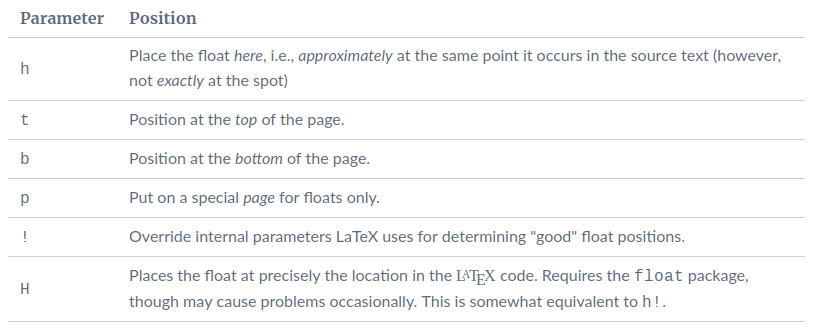
\includegraphics[width=1.0\textwidth]{figurelatex.png}
 \caption{}
\end{figure}
\end{document}
